\documentclass[11pt]{article}
\usepackage[margin=1 in, letterpaper]{geometry}
\usepackage{fontspec, graphicx, amsmath, amssymb, amsthm, array, physics, enumitem, cancel, multicol, float, bm}
\usepackage[dvipsnames]{xcolor}

\setmainfont{Linux Libertine O}
\setsansfont{Linux Biolinum O}
\setmonofont{Latin Modern Mono}
\setmathrm{Latin Modern Math}
\theoremstyle{definition}
\newtheorem{theo}{\color{Maroon} Theorem}
\newtheorem{defin}[theo]{\color{Maroon} Definition}
\newtheorem{example}[theo]{\color{Maroon} Example}
\newtheorem{prob}[theo]{\color{Maroon} Problem}
% \newtheorem{example}[section]{\color{Maroon} Example}
\usepackage{lscape}
\theoremstyle{remark}
\newtheorem*{soln}{\color{Maroon} Solution}
\usepackage{latexsym, marvosym}

\newcommand{\convas}{\xrightarrow{\text{a.s.}}}
\newcommand{\convprob}{\xrightarrow{\mathbb{P}}}
\newcommand{\convdist}{\xrightarrow{d}}

\newcommand{\R}{\mathbb{R}}
\newcommand{\Q}{\mathbb{Q}}
\newcommand{\Z}{\mathbb{Z}}
\newcommand{\N}{\mathbb{N}}
\newcommand\independent{\protect\mathpalette{\protect\independenT}{\perp}}
\def\independenT#1#2{\mathrel{\rlap{$#1#2$}\mkern2mu{#1#2}}}

%%%%%%%%%%%%%%%%%%% Statistics %%%%%%%%%%%%%%%%%%%%
\newcommand{\E}[1]{\mathbb{E}\left[ #1 \right]}
\newcommand{\Prob}[1]{\mathbb{P}\left[ #1 \right]}
\newcommand{\cov}[2]{\textnormal{Cov}\left[ #1, #2 \right]}
\renewcommand{\var}[1]{\textnormal{Var}\left[ #1 \right]}
% \renewcommand{\var}{\textnormal{Var}}
% \newcommand{\cov}{\textnormal{Cov}}
\newcommand{\Unif}{\textnormal{Unif}}
\newcommand{\Norm}{\mathcal{N}}
\newcommand{\Bin}{\textnormal{Bin}}
\newcommand{\Beta}{\textnormal{Beta}}
\newcommand{\Bern}{\textnormal{Bern}}
\newcommand{\Geom}{\textnormal{Geom}}
\newcommand{\FS}{\textnormal{FS}}
\newcommand{\Expo}{\textnormal{Expo}}
\newcommand{\DUnif}{\textnormal{DUnif}}
\newcommand{\Pois}{\textnormal{Pois}}
\newcommand{\NBin}{\textnormal{NBin}}
\newcommand{\HGeom}{\textnormal{HGeom}}
\newcommand{\Gam}{\textnormal{Gamma}}
\newcommand{\Mult}{\textrm{Mult}}
\newcommand{\iidsim}{\overset{\text{iid}}{\sim}}

%%%%%%%%%%%%%%%%%%%%%%%%%%%%%%%%%%%%%%%%%%%%%%%%%%%%%%%%%%%%%%%%%%%%
\newcommand{\inserttitle}{2015 Finals Solution}
\newcommand{\insertauthor}{Max Guo \& Seung Hwan An}
\newcommand{\insertcourse}{STAT 110}
%%%%%%%%%%%%%%%%%%%%%%%%%%%%%%%%%%%%%%%%%%%%%%%%%%%%%%%%%%%%%%%%%%%%

\usepackage{fancyhdr}
\setlength{\headheight}{15pt}
\pagestyle{fancy}
\fancyhf{}
\fancyhead[C]{\thepage}
\fancyhead[L]{\inserttitle}
\fancyhead[R]{\insertauthor}

%%%%%%%%%%%%%%%%%%%%%%%%%%%%%%%%%%%%%%%%%%%%%%%%%%%%%%%%%%%%%%%%%%%%

\begin{document}

{\noindent\Huge\bf  \\[0.1\baselineskip] {\inserttitle }}\\[2\baselineskip]
{{\bf \insertcourse}\\ {\textit{December 6, 2021}}} \hfill {\large \textsc{\insertauthor}}
\smallskip

\begin{prob} A crime has been committed in a certain country. The perpetrator is one (and only one) of the $n$ men who live in the country. Initially, these $n$ men are all equally likely to be the perpetrator. An eyewitness then reports that the crime was committed by a man with six fingers on his right hand. Let $p_0$ be the probability that an innocent man has six fingers on his right hand, and $p_1$ be the probability that the perpetrator has six fingers on his right hand, with $p_0 < p_1$. (We may have $p_1 < 1$, since eyewitnesses are not $100\%$ reliable.) Let $a = p_0 / p_1$ and $b = (1-p_1)/(1 - p_0)$.\\

\noindent
Rugen lives in the country. He is found to have six fingers on his right hand.

\begin{enumerate}[label = (\alph*)]
    \item Given this information, what is the probability that Rugen is the perpetrator? Simplify fully, and express your answer in terms of $n$ and $a$.
    
    \begin{soln} Let $S$ be the event that Rugen has six fingers, and let $G$ be the event that Rugen is guilty. Then we have the following, by Bayes' Rule:
    \begin{align*}
        P(G | S) &= \frac{P(S|G)P(G)}{P(S)} \\
        &= \frac{P(S|G)P(G)}{P(S|G)P(G) + P(S|G^C)P(G^C)} \\
        &= \frac{p_1 \cdot 1/n}{p_1 \cdot 1/n + p_0 \cdot \frac{n-1}{n}} \\
        &= \frac{1}{1 + (n-1)a}
    \end{align*}
    \end{soln}
    
    \dotfill
    
    \item Now suppose that all $n$ men who live in the country have their hands checked, and Rugen is the \textit{only} one with six fingers on his right hand. Given this information, what is the probability that Rugen is the perpetrator? Simplify fully, and express your answer in terms of $n$, $a$, and $b$.
    
    \begin{soln}
    Among the $n-1$ people who are not Rugen, let $F_i$, $1 \le i \le n-1$, be the event that the $i$th person has five fingers. Then we have that:
    \begin{align*}
        P(G | F_1, \dots, F_{n-1}, S) &= \frac{P(S, F_1, \dots, F_{n-1}|G)P(G)}{P(S, F_1, \dots, F_{n-1}|G)P(G) + P(S, F_1, \dots, F_{n-1}|G^C)P(G^C)} \\
        &= \frac{p_1(1 - p_0)^{n-1}\cdot \frac{1}{n}}{p_1(1 - p_0)^{n-1}\cdot \frac{1}{n} + p_0(1-p_1)(1-p_0)^{n-2}(1 - \frac{1}{n})} \\
        &= \frac{1}{1 + ab(n-1)}
    \end{align*}
    \end{soln}
\end{enumerate} 

\end{prob}

\pagebreak

\begin{prob} Let $X,Y,Z$ be i.i.d. with a continuous distribution. Write the most appropriate of $\leq, \geq, = $, or $?$ in each blank.

\begin{enumerate}[label = (\alph*)]
    \item $P(X<Y<Z) = 1/6$. 
    
    \begin{soln} $P(X<Y<Z)$ is equal to $1/3!=1/6$ because $X,Y,Z$ are i.i.d. and continuous, so the probability of ties are $0$.
    \end{soln}
    
    \dotfill
    
    \item $P(X > 1) ? E[X]$. 
    
    \begin{soln} If $X$ is nonnegative, this is $\le$ be Markov's inequality. Otherwise, $X$ could be negative all the time, resulting in $>$.
    \end{soln}
    
    \dotfill
    
    \item $P \left( \sum_{k=0}^{2015} \left(\frac{X^2+1}{X^2+2}\right)^k > 3 \right) \leq P( X > 2 )$.
    
    \begin{soln}
    Note that 
    \begin{align*}
        \left(\frac{X^2+1}{X^2+2}\right)^k &\le \frac{1}{1 - \frac{X^2+1}{X^2+2}} \\
        &= X^2 + 2.
    \end{align*}
    So if the nasty sum is $>3$, then we must have $X^2 + 2 > 3$, so $X^2 > 1$. Implications give us probability inequalities!
    \end{soln}
    
    \dotfill
    
    \item $\E{\sqrt{X^2 + Y^2}} \le \sqrt{E[X^2] + E[Y^2]}$. 
    
    \begin{soln} Let $Z = X^2 + Y^2$. Then this is comparing $E[\sqrt{Z}]$ with $\sqrt{E[Z]}$, which is done via Jensen's (square root is concave).
    \end{soln}
    
    \dotfill
    
    \item $\var{Y^2|Z} \ge \var{X^2|X}$.
    
    \begin{soln}
    The latter has zero variance.
    \end{soln}
    
    \dotfill
    
    \item $\var{X - 2Y + 3Z} = 14\var{X}$.
    
    \begin{soln} By independence and properties of variance, the left hand side is $\var{X} + 4\var{Y} + 9\var{Z}$, and by i.i.d. we obtain equality.
    \end{soln}
    
\end{enumerate}

\end{prob}

\pagebreak

\begin{prob} Emails arrive in an inbox according to a Poisson process of rate $\lambda$ emails per hour.

\begin{enumerate}[label = (\alph*)]
    \item Find the name and parameters of the conditional distribution of the number of emails that arrive in the first 2 hours of an $8$-hour time period, given that exactly $n$ emails arrive in that time period.
    
    \begin{soln} 
    The joint distribution of the arrival times in the $8$ hour period given that $n$ emails arrive in the $8$ hours is distributed the order statistics of $n$ i.i.d. Uniform(0, 8) random variables. If we treat the $8$ hours as four two hour blocks, then we see that this has a Binomial distribution with parameters $n, 1/4$. (See Theorem 13.2.3)
    \end{soln}
    
    \dotfill
    
    \item Each email is legitimate with probability $p$ and spam with probability $q = 1 - p$, independently. Find the name and parameters of the conditional distribution of the number of legitimate emails that arrive in an $8$-hour time period, given that exactly $s$ spams arrived in that time period.
    
    \begin{soln} By Poisson Process Thinning or the Chicken Egg Story, the ``spam" and ``legitimate" email arrival counts are independent of each other! The legitimate emails are distributed $\Pois(8\lambda p)$.
    \end{soln}
    
    \dotfill
    
    \item Reading an email takes a random amount of time, with mean $\mu$ hours and standard deviation $\sigma$ hours. These reading times are i.i.d. and independent of the email arrival process. Find the (unconditional) mean and variance of the total time it takes to read all the emails that arrive in an $8$ hours time period.
    
    \begin{soln} Let $R_i$ be the $i$th reading time. We have by Adam's and Eve's laws:
    \begin{align*}
        \E{\sum_{i=1}^N R_i}
        &= \E{\E{\sum_{i=1}^N R_i | N}} \\
        &= \E{N\mu} \\
        &= 8\lambda \mu.
    \end{align*}
    \begin{align*}
        \var{\sum_{i=1}^N R_i} &= \E{\var{\sum_{i=1}^N R_i | N}} + \var{\E{\sum_{i=1}^N R_i | N}} \\
        &= 8\lambda \sigma^2 + 8\lambda \mu^2
    \end{align*}
    \end{soln}
    
\end{enumerate}

\end{prob}

\pagebreak

\begin{prob} There are $k$ distinguishable balls and $n$ distinguishable boxes. The balls are randomly placed in the boxes, with all $n^k$ possibilities likely.

\begin{enumerate}[label = (\alph*)]
    \item Find the expected number of empty boxes (fully simplified, \textit{not} as a sum).
    
    \begin{soln} 
    Using indicator variables $I_1, \dots, I_n$ we represent the $i$th box being empty, we obtain:
    \begin{align*}
        P(I_j = 1) &= \left(\frac{n-1}{n}\right)^k
    \end{align*}
    Summing $n$ of them and using linearity:
    \begin{align*}
        \E{\sum_{j=1}^n I_j} = \frac{(n-1)^k}{n^{k-1}}
    \end{align*}
    \end{soln}
    
    \dotfill
    
    \item Find the probability that at least one box is empty. Express your answer as a sum of at most $n$ terms.
    
    \begin{soln} We use the Inclusion Exclusion principle, which is hinted by the ``at most $n$ terms":
    \begin{align*}
        P(\text{at least one box empty}) &= P(\text{one box empty}) - P(\text{two boxes empty}) + P(\text{three boxes empty}) - \dots \\
        &= \sum_{i=1}^n (-1)^{i+1}\binom{n}{i}\left(\frac{n-i}{n}\right)^k
    \end{align*}
    \end{soln}
    
    \dotfill
    
    \item Now let $n = 1000$, $k = 5806$. The expected number of empty boxes is then approximately $3$. Find a good approximation for the probability that at least one box is empty (give a decimal approximation). You can use the handy fact $e^3 \approx 20$.
    
    \begin{soln}
    For large $n$, this is the story of a Poisson approximation. We have that the number of empty boxes is distributed approximately $\Pois(3)$, and the probability there is no boxes empty is $e^{-3} \approx 0.05$, so our desired probability is $0.95$.
    \end{soln}
    
\end{enumerate}

\end{prob}

\pagebreak

\begin{prob}
\begin{enumerate}[label = (\alph*)]
    \item You are given an opportunity to bid on a mystery box containing a mystery prize! The value of the prize is completely unknown, except that it is worth at least nothing, and at most a million dollars. So the true value $V$ of the prize is considered to be Uniform on [0,1] (measured in millions of dollars). You can choose to bid any nonnegative amount $b$ (in millions of dollars). If $b < V/4$, then your bid is rejected and nothing is gained or lost. If $b \ge V/4$, then your bid is accepted and your net payoff is $V − b$ (since you pay $b$ to get a prize worth $V$). Find your expected payoff as a function of $b$ (be sure to specify it for all $b \ge 0$). Then find the optimal bid $b$, to maximize your expected payoff.
    
    \begin{soln} We calculate the expected payoff as the following:
    \begin{align*}
    \E{V - b | b \ge V/4}P(b \ge V/4)
    &= \E{V - b | V \le 4b}P(V \le 4b)
    \end{align*}
    Note that if $b \ge 1/4$, then $P(V \le 4b) = 1$, and $\E{V-b | V \le 4b} = \E{V - b} = 1/2 - b$. If $b < 1/4$, then $P(V \le 4b) = 4b$ by the Uniform CDF, and $\E{V - b | V \le 4b}P(V \le 4b) = (2b - b)4b = 4b^2$. Optimizing this, we obtain $b = 1/4$.
    \end{soln}
\end{enumerate}

\end{prob}

\pagebreak

\begin{prob}Suppose that the time until a radioactive particle decays is $\Expo(\lambda)$.

\begin{enumerate}[label = (\alph*)]
    \item Show that for $c$ a small, positive constant, the probability that such a particle decays in the time interval $(t, t + c]$, given that it has survived until time $t$, does not depend on $t$ and is approximately proportional to $c$. Hint: $e^x \approx 1 + x$ if $x \approx 0$.
    
    \begin{soln} Exponential is memoryless, so $T -t | T > t$ is still $\Expo(\lambda)$. Thus, $P(t < T \le t + c | T > t) = 1 - e^{-\lambda c} \approx \lambda c$, which is proportional to $c$.
    \end{soln}
    
    \dotfill
    
    \item Consider $3$ radioactive particles, with i.i.d. times until decay $T_1, T_2, T_3 \sim \Expo(\lambda)$. Let $X$ be the last time at which one of the particles decays. Find $\E{X}$. (Simplify.)
    
    \begin{soln} Let $X = X_1 + X_2 + X_3$, where each $X_i$ is the time in between the $i-1$th particle decay and the $i$th particle decay. By minimum independent Expos, 
    \begin{align*}
        \E{X} = \frac{1}{3\lambda} + \frac{1}{2\lambda} + \frac{1}{\lambda} = \frac{11}{6\lambda}.
    \end{align*}
    \end{soln}
    
\end{enumerate}

\end{prob}

\pagebreak

\begin{prob} Let $X,Y,Z,W \sim \Norm(0,1)$ be i.i.d., $\Phi$ be the $\Norm(0,1)$ CDF.

\begin{enumerate}[label = (\alph*)]
    \item Find an expression for $\E{\Phi(Z)e^Z}$ as an unsimplified integral.
    
    \begin{soln}
    By LOTUS, we have:
    \[
    \E{\Phi(Z)e^Z} = \int_{-\infty}^\infty \Phi(z)^{z}\varphi(z)\mathrm dz,
    \]
    where $\varphi(z)$ is the $\mathcal N(0, 1)$ PDF.
    \end{soln}
    
    \dotfill
    
    \item Find $\E{\Phi(Z)}$ and $E[e^Z]$.
    
    \begin{soln}
    $\Phi(Z)$ is Uniform by UoU, so $\E{\Phi(Z)} = 1/2$. $\E{e^Z}$ reminds us of the MGF of the standard normal, which is $E[e^{tZ}] = e^{t^2/2}$. Here $t = 1$, so $E[e^Z] = e^{1/2}$.
    \end{soln} 
    
    \dotfill
    
    \item Find $P(X + Y < Z + W + 1)$ in terms of $\Phi$. (Simplify fully.)
    
    Note that $X + Y - Z - W$ is distributed $\Norm(0, 4)$, so 
    \[
    P\left(\frac{X + Y - Z - W}{2} < \frac{1}{2}\right) = \Phi\left(\frac{1}{2}\right).
    \]
    
\end{enumerate}

\end{prob}

\pagebreak

\begin{prob}

The problem is attached:

\begin{figure}[h!]
    \centering
    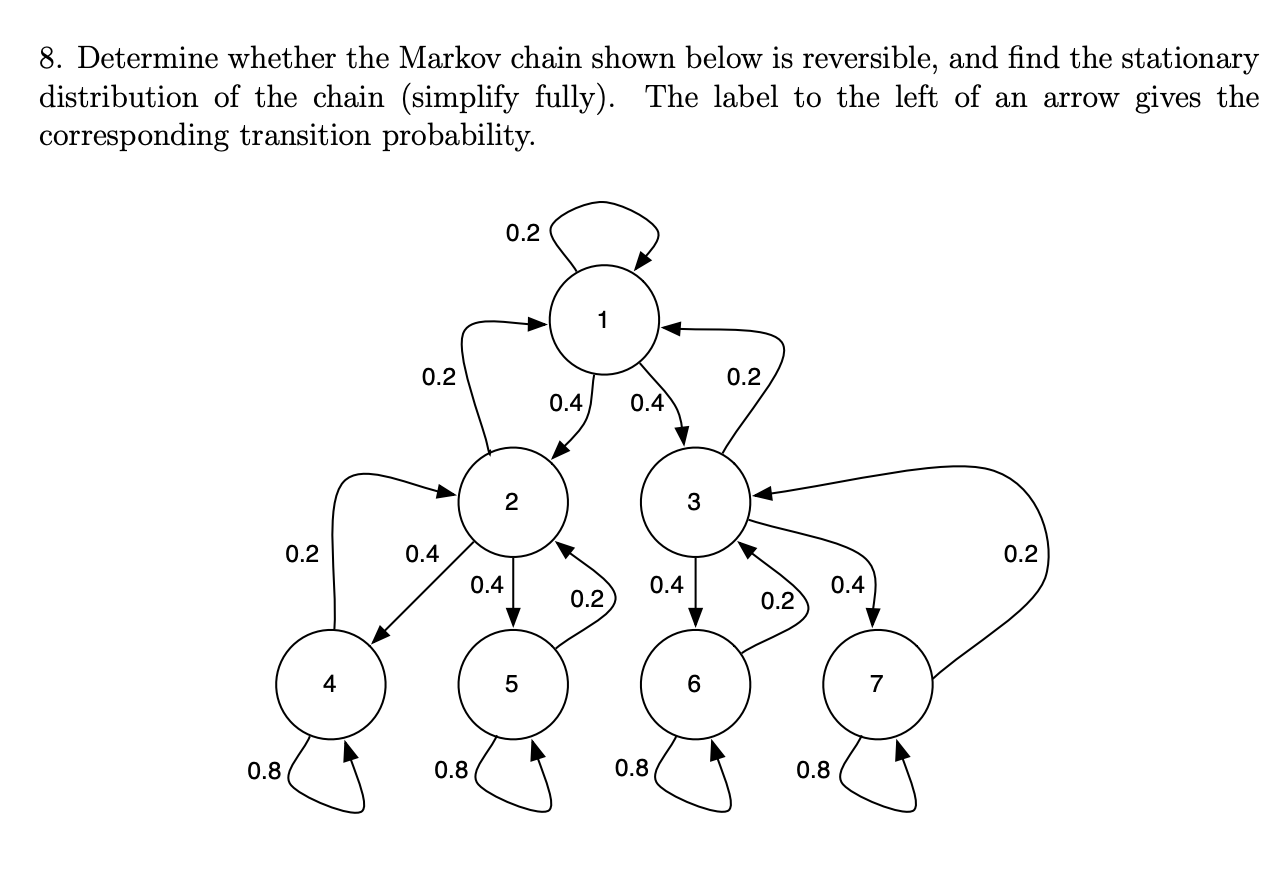
\includegraphics[width=0.8\textwidth]{image/2015p8.png}
\end{figure}

\begin{soln}
We set $s_1 = 1$ (unnormalized), then find that $s_2 = 2$ if we want to satisfy the reversibility criterion for $s_1p_{12} = s_2p_{21}$, and similarly $s_4 = 4$ for $s_2p_{24} = s_4p_{42}$. By symmetry, $s_3 = 2$ and $s_5 = s_6 = s_7 = 4$. Normalizing, we obtain:
\[
[1/21, 2/21, 2/21, 4/21, 4/21, 4/21, 4/21]
\]
and we check that this chain indeed satisfies all reversibility conditions.
\end{soln}

\end{prob}


\end{document}